\section{The Bias Parameter}

In our analysis, we assumed $\gamma = 0$ for simplicity, but the $\gamma$ parameter
seems to be a promising knob to tune the performance of PoEM. While we leave the
analytic treatment of the optimal $\gamma$ for future work, we note here that,
for a given value of $g$, the delay of the system behaves as illustrated in Figure~\ref{fig:bias}
for varying values of $\gamma$. We believe that this graph behaves convexly for
small values of $\gamma$, whereas, for $\gamma \to \infty$, the delay converges to
the behavior of Bitcoin. Indeed, if $\gamma$ is made sufficiently large, the bias
parameter dominates against the $-\lg\frac{H(B)}{T}$ term, and the system behaves
as if each block counts the same amount of work, converging at the limit to the
longest chain rule.

\iftwocolumn
\begin{figure}[h]
    \centering
    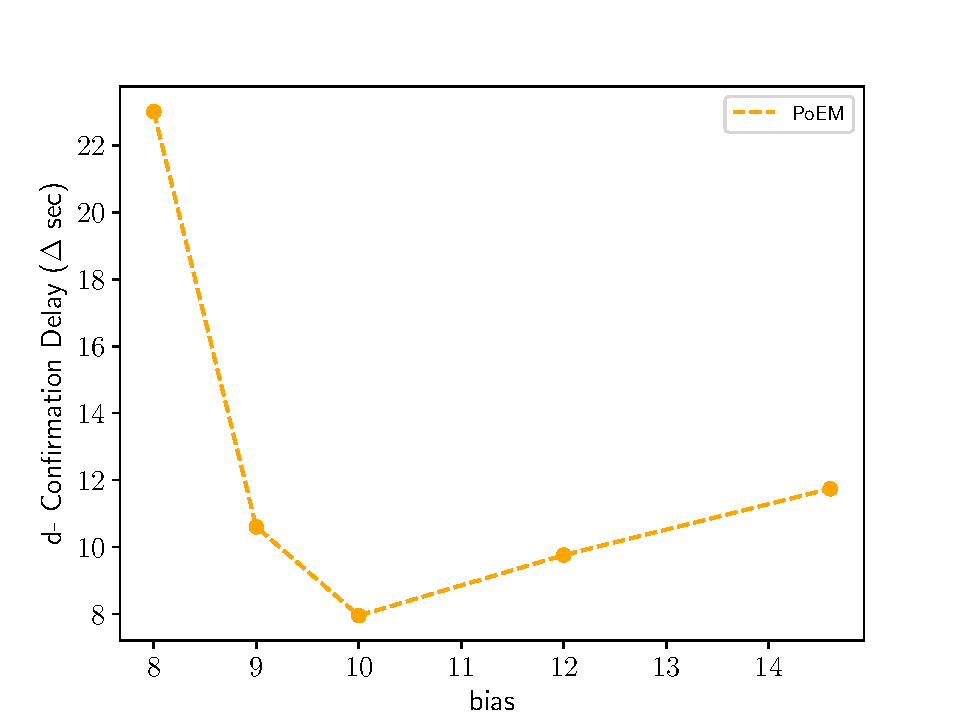
\includegraphics[width=\columnwidth,keepaspectratio]{figures/gamma.pdf}
    \caption{Confirmation delay $d$ (measured in network delay $\Delta$ units) vs. the bias $\gamma$. The bias, $\gamma$ was experimentally optimized for the $g = 0.99$ which showed the lowest confirmation delay in Bitcoin.
    }
    \label{fig:bias}
\end{figure}
\else
\begin{figure}[h]
    \centering
    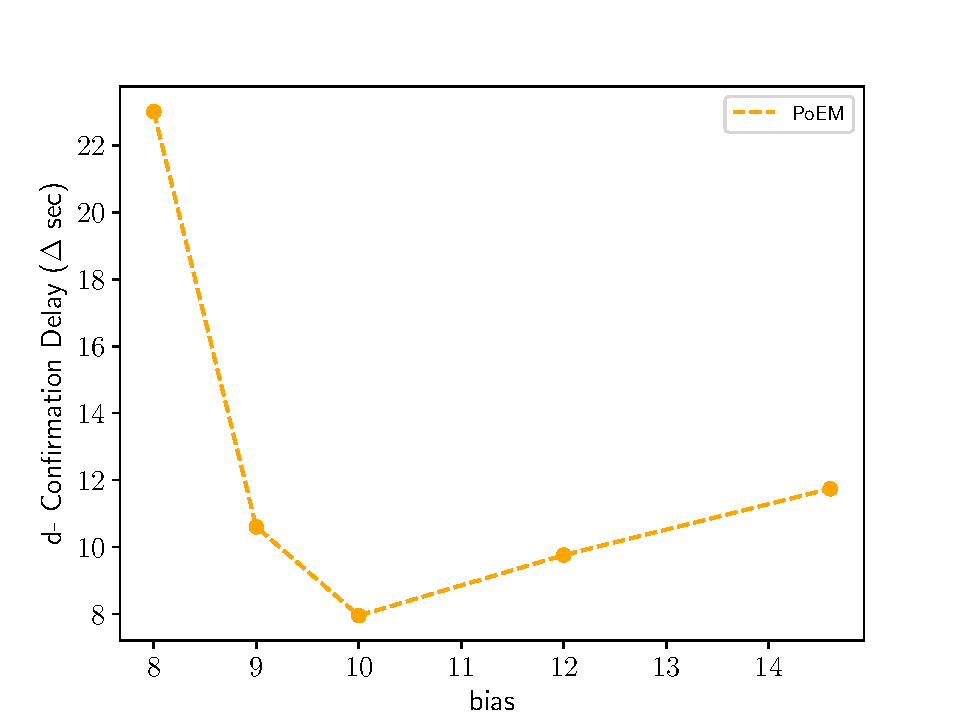
\includegraphics[width=0.8 \columnwidth,keepaspectratio]{figures/gamma.pdf}
    \caption{Confirmation delay $d$ (measured in network delay $\Delta$ units) vs. the bias $\gamma$. The bias $\gamma$ was experimentally optimized for $g = 0.99$ which showed the lowest confirmation delay in Bitcoin.
    }
    \label{fig:bias}
\end{figure}
\fi